\chapter{Analyse der Fachdomäne Hochschulsport} 
\label{ch:hochschulsport} 
Die Aufgaben und Anforderungen, die an deutsche Hochschulen gestellt werden sind vielfältig und erstrecken sich in viele verschiedene Bereiche. Neben den Kernaufgaben der universitären Lehre und wissenschaftlichen Forschung gehört es auch zu den Aufgaben, das studentische Leben in sozialen und gesellschaftlichen Belangen zu unterstützen und zu fördern. Neben Einrichtungen wie dem Studierendenwerk oder dem Allgemeinen Studierendenausschuss (AStA) ist auch der Hochschulsport eine Einrichtung, die unterschiedlichste Aufgaben im Umfeld der Fachhochschulen und Universitäten übernimmt. Im Vergleich zu amerikanischen Universitäten erscheint der Hochschulsport in Deutschland oft als rein schmückendes Element. Allein der Mitteleinsatz für die Erreichung eines hohen Niveaus des Hochschulsportprogrammes in Amerika übersteigt die Ausgaben um ein Vielfaches. In deutschen Hochschulsporteinrichtungen lagen die Aufwendungen für Personal-und Sachmittel im Jahre 2004 für Universitäten bei etwa 300.000€ und bei Fachhochschulen bei rund 30.000€ \cite[vgl. ][S.9]{Hachmeister.2004}. 
Der erste Teil dieser Diplomarbeit soll ein Verständnis für die Domäne Hochschulsport und deren Entwicklung, Organisationsformen, Aufgaben sowie Probleme und Herausforderungen vermitteln.

\section{Historische Entwicklung des Hochschulsports}
Das Sporttreiben an deutschen Hochschulen begann zwar nicht erst nach dem zweiten Weltkrieg, die historische Betrachtung soll sich hier jedoch auf die Zeit zwischen 1948 und 2009 beschränken, um den Rahmen der Arbeit nicht zu sprengen. Da die Organisation von Bildung in die Zuständigkeit der Bundesländer fällt, hat die Entwicklung durchaus unterschiedliche Wege genommen. Ich konzentriere mich in diesem Fall auf den geschichtlichen Rückblick mit dem Schwerpunkt NRW, da hier die umfangreichsten Dokumentationen verfügbar waren. 
Der 1999 von von 29 Bildungsministern initiierte Bologna-Prozess zur Schaffung eines einheitlichen Hochschulraums \cite*[vgl.][]{Zandonella.2005}
 
\subsection{Hochschulsport heute}
Durch die gesetzliche Verankerung im Hochschlrahmengesetz und die Festschreibung in den einzelnen Landeshochschulgesetzen hat sich eine vorerst gesicherte Grundlage zur Förderung des Sports an Hochschulen manifestiert. Die einzelnen Hochschulsporteinrichtungen (HSP) besitzen eine gefestigte Position im Hochschulkontext und müssen nicht mehr um ihre grundlegende Daseinsberechtigung kämpfen. Trotz gesicherter Grundlagen haben etwa 40  \% der Hochschulsporteinrichtungen mit Mittelkürzungen zu kämpfen \cite[][S.9]{Hachmeister.2004}.
Das Grundanliegen des HSP ist und bleibt jedoch die Förderung des Sporttreibens der Studierenden, die sich in speziellen Lebensphasen befinden und durch besondere Umstände geprägt sind. Das diese nicht generalisiert werden können, lässt sich leicht nachvollziehen, da unterschiedliche Studiengänge, Wohnumstände und Studiumsformen die Lebensphase in sehr heterogener Weise beeinflussen können. Der Einfluss auf den Hochschulsport und im speziellen auf die Akzeptanz und Teilnahme lässt sich an folgenden Kriterien festmachen, die speziell bei der Hochschulsportorganisation explizit berücksichtigt werden müssen:

\begin{enumerate}
	\item Sportinteresse des Studierenden
	\item Ort der Sporteinrichtungen
	\item Soziale Kontakte
	\item Belastungen und Entbehrungen
\end{enumerate}

Somit ergibt sich für den Hochschulsport heute die besondere Herausforderung den Bedürfnissen der Studierenden gerecht zu werden und ihnen die Gelegenheit zu geben, gemäß ihrer Interessen und Vorstellungen Sport treiben zu können. \\
Der bereits erwähnte Bologna-Prozess führte allerdings zu weiteren Herausforderungen im Verhältnis Hochschulsport-Studierende \cite[vgl. ][S.7]{Berthold.2007}. Die Verkürzung der Studienzeit führte zu einem strenger vorgegebenen Studienplan und einer deutlichen Verknappung der persönlichen Gestaltungs- und Freizeitmöglichkeiten. Diese Faktoren beeinflussen die Möglichkeiten der Studierenden an der Teilnahme im Hochschulsport erheblich, sodass sich des Hochschulsportprogramm diesen speziellen Anforderungen noch stärker durch mehr Flexibilität und neue Angebotsformen stellen muss.
\\
Neben dem Einfluss des Bologna-Prozesses auf die Studierenden zeigt die einher gehende Restrukturierung der Hochschulen auch direkten Einfluss auf die Hochschulsporteinrichtungen. Durch die Messung der Hochschulen anhand ihrer Erfolge in den Kernprodukten, schrumpfen die Möglichkeiten für zusätzliche Angebote, was sich auch in der Bereitstellung der Finanz- und Sachmittel widerspiegelt. \citeauthor{Berthold.2007} sehen dabei folgende vier Bedrohungen für den Hochschulsport:
\begin{enumerate}
\item \textbf{Einsparungen:} Linear an der allgemeinen Sparbemühungen beteiligt zu sein, kann den Hochschulsport bei bisher generell eher magerer Ausstattung vollends marginalisieren.
\item \textbf{Leistungsorientierung:} je mehr die Hochschulen von den Länder über eine leistungsorientierte Mittelverteilung finanziert werden, desto eher könnten die Hochschulen einen Anreiz empfinden, sich auf die in Kennzahlen ausgedrückten Kernleistungen zu konzentrieren.
\item \textbf{Studienzeitverkürzung:} Wenn im Rahmen der Umstellung auf gestufte Studiengänge tatsächlich eine striktere Einhaltung der Regelstudienzeit erreicht werden sollte, dann werden die Studierenden intensiver studieren. Das dürft dazu führen, dass sie weniger Zeit für Mitwirkung am Sport zur Verfügung haben und das sie sich weniger ehrenamtlich in der Betreuung engagieren.
\item \textbf{Studiengebühren:} Ist bereits das Studium kostenpflichtig, so werden sich die Studierenden eher fragen, ob sie for Sportangebote zusätzlich zahlen wollen. Sollten sie in den Konflikt zwischen intensiver Belastung durch das Studium und seiner Finanzierung durch Nebentätigkeiten geraten, so dürfte die Betätigung im Sport das sein, was geopfert würde.
\end{enumerate}
\cite[siehe ][S.16]{Berthold.2007}
Nach der bundesweiten Abschaffung der Studiengebühren ist diese Bedrohung zur Zeit nicht mehr so prekär, wie einst angenommen.
\\

Neben den Studierenden gehören aber zunehmend auch andere Personenkreise zur Zielgruppe des Hochschulsports. Besonders die Bediensteten der Hochschule werden zunehmend in den Programmen mit speziellen Angeboten angesprochen. Speziell im Bereich Gesundheitssport haben sich verschiedene Programme an den Hochschulen oder auch durch übergeordnete Gremien, wie den Allgemeinen Deutschen Hochschulsportverband (adh), etabliert. Das Angebot ist dabei sehr unterschiedlich und stark abhängig von den verfügbaren Ressourcen, erstreckt sich von der Teilnahme am allgemeinen Programm über spezielle Bediensteten Kurse bis hin zur individuellen Betreuung am Arbeitsplatz im Büro. [\textbf{Entwicklung von Gesundheitskursen}] Die Nachfrage nach gesundheitsfördernden Maßnahmen dieser Art erfreut sich derzeit einer hohen Nachfrage und wird sowohl vom adh als auch von den Hochschulsporteinrichungen in der Mehrheit als aktuelle und zukünftige Kernaufgabe des Hochschulsports gesehen \cite[vgl.][]{Baumgarten.2009}.
Die Potenziale des Hochschulsports, der wichtige Beitrag zur sozialen und integrativen Unterstützung sowie die positiven, gesundheitsfördernden Effekte auf die Studierenden werden von \cite{Goring.2010} zusammen gefasst. 
\\

Neben den Bediensteten lassen sich aber auch externe Teilnehmer als weitere Zielgruppe bestimmen. Die Einbindung dieser Personenkreise unterscheidet sich am stärksten in den unterschiedlichen Einrichtungen und birgt großes Potenzial und Gefahr gleichzeitig. Je nach Organisationsform stehen dem Hochschulsport ganz unterschiedliche Möglichkeiten offen aber auch das regionale Umfeld muss hier analysiert werden. Mit der Öffnung des Hochschulsports für externe Teilnehmer begibt man sich in direkte Konkurrenz mit kommerziellen Anbietern. Die Integrationsformen variieren von Kooperationen mit Vereinen, Firmen im Rahmen von Betriebssportangeboten, Rehakliniken und Gesundheitszentren bis hin zur freien Öffnung für Jedermann. Allgemein lässt sich jedoch beobachten, dass diese Gruppe vor allem dann angesprochen wird, wenn eine Auslastung durch Bedienstete und Studierende nicht möglich ist. Im Bereich Organisationsformen werde ich auf die Unterschiede noch detaillierter eingehen.  
\section{Typische Aufgaben}
\paragraph*{Dauerhafte Motivation und Möglichkeit zum Sporttreiben} Ausgleich zu den alltäglichen und universitären Belastungen
\paragraph*{Gesundheitsförderung und entwickeln einer umfassenden Mitverantwortung für eine gesunde Lebensführung}
\paragraph*{Erwerb von Soft-Skills}
\paragraph*{Bereicherung des studentischen Lebens an der Hochschule und Integration über den Sport}
\paragraph*{Ausbildung von Übungsleitern}
\paragraph*{Profilbildung Hochschule}
\paragraph*{Erprobung neuer Trends}
\paragraph*{Unterstützung von studierenden Spitzensportlern bei der Vereinbarkeit von Studium und Sport}

\section{Organisationsformen}
Wie bereits bemerkt lassen sich unterschiedliche Organisationsformen der Hochschuleinrichtungen finden. \citet*[S. 15]{Radde.1996} gliedert diese in drei Formen:
\paragraph*{Die zentralen Einrichtungen}
Sie ist die am häufigsten anzutreffende Organisationsform seit der Festschreibung des Hochschulsportes im Hochschulrahmengesetz. Unabhängig von einem Fachbereich und direkt dem Senat unterstellt hat sie die Aufgabe den Hochschulsport eigenständig zu organisieren und zu verwalten.

\paragraph*{Die in das Aufgabenfeld der Institute für Sportwissenschaft integrierte Organisation des Hochschulsports}
Diese enge Verbindung mit der Sportlehrer/innenausbildung kann sich auf das Hochschulsportangebot äußerst positiv auswirken, bringt aber auch durch notwendige „Prioritätensetzungen“ die Gefahr der Benachteiligung mit sich. Nicht selten kommt es zu konkurrierenden Ansprüchen bei Hallenzeiten, Personal und Finanzierungen.

\paragraph*{Der durch studentische Selbstverwaltung organisierten Hochschulsport}
Eine solche Form hat sich vor allem an kleineren Hochschulen bzw. Fachhochschulen etabliert, wo keine hauptamtlichen Sportlehrer/innen zur Verfügung stehen. Die Übernahme der Verantwortung durch Studierende begrenzt die Leistungsfähigkeit der Einrichtung, ermöglicht aber gleichzeitig den Erwerb von Kompetenzen für Studierende, die in anderen Organisationsformen nicht möglich sind. 

\section{Befragung ausgewählter Standorte}
Im Rahmen der Anforderungsanalyse an ein Hochschulsportverwaltungssystem wurde eine Befragung an \textbf{sieben} Hochschulsporteinrichtungen durchgeführt zur Ermittlung existierender Systeme, wichtiger Kernfunktionen und Prioritäten (Tabelle~\ref{BefragungHochschulen}).

\begin{table}[h]
\centering
\resizebox{\textwidth}{!}{%
\begin{tabular}{|l|l|l|l|l|l|l|l|}
\hline
\textbf{Name}                     & \textbf{Bundesland} & \textbf{Typ} & \textbf{TN/Jahr} & \textbf{Mitarbeiter} & \textbf{Übungsleiter} & \textbf{Kurse/Jahr} \\ \hline
Hochschulsport Göttingen          & Niedersachsen       & übergreifend & 15.000           & 20                   & 150                   & 550                 \\ \hline
Hochschulsport Münster            & Nordrhein-Westfalen & übergreifend & 20.000           & 30                   & 500                   & n.a.                \\ \hline
Hochschulsport Osnabrück          & Niedersachsen        & übergreifend & 3.000            & 10                   & 100                   & 380                 \\ \hline
Hochschule Darmstadt              & Hessen              & exklusiv     & 1.000            & 2                    & 40                    & 120                 \\ \hline
Hochschulsport Uni des Saarlandes & Saarland            & übergreifend & 4.000/Woche      & 8                    & 150                   & 500                 \\ \hline
Hochschulsport Hamburg            & Hamburg             & übergreifend & 10.000/Pers.     & 15                   & 350                   & 1400                \\ \hline
Hochschulsport Berlin             & Berlin              & übergreifend & 18.000           & 20                   & 300                   & 1150                \\ \hline
\end{tabular}}
\caption{Übersicht befragter Hochschulen}
\label{BefragungHochschulen}
\end{table}

Die Stichprobe stell einen Ausschnitt unterschiedlicher Hochschulsportgrößen, Bundesländer dar. Alle der befragten Einrichtungen gaben dabei an, als zentrale Einrichtung an der Universität bzw. Hochschule organisiert zu sein. Die Angaben zu den Teilnehmerzahlen im Jahr konnte nicht immer genau beantwortet werden, was auf folgende Gründe zurück zu führen ist:
\begin{itemize}
\item Die Teilnehmerzahlen können unterschieden werden nach Personenanzahl, Anzahl der Besucher je Kurs und Anzahl der Besucher je Kurstermin
\item Die verwendeten Systeme konnten keine genaue Aufschlüsselung darübermachen, wie viele Personen und Kursbesuche in einem Definierten Zeitraum stattfinden
\item Anmeldefreie Angebote werden in der Regel nicht mit Teilnehmerzahlen erfasst
\end{itemize}

Die daraufhin erfolgen Angaben sollen in diesem Fall als Schätz- und Näherungswerte dienen, um den Nutzerkreis etwa beurteilen zu können. 

Die Befragung gliederte sich in \textbf{X} Teile:

\begin{enumerate}
\item Allgemeine Angaben zur Hochschulsporteinrichtung (siehe Tabelle ~\ref{BefragungHochschulen})
\item Was für eine System wird aktuelle verwendet und wie zufrieden ist der HSP mit der aktuellen Lösung
\item Bewertung der Wichtigkeit einzelner Funktionalitäten für den HSP
\item Zusätzliche Anmerkungen
\end{enumerate}

\subsection{Aktuelle Lösungen}
Um einschätzen zu können, mit Hilfe welcher Systeme die Organisation erfolgt, wurde ermittelt wie viele Einrichtungen eine spezielle Software für die Verwaltung des Hochschulsports nutzen. Der überwiegende Teil der Befragten mit 85.71 \% gab an eine spezielle Software zu verwenden und nur 14,29 \% nutzten eine andere Lösung in Form von Microsoft Excel und der Hochschulwebsite. Bei der Verwendung einer Hochschulsportverwaltungssoftware ergab sich ein Verhältnis von 66,66 \% zum System BuchSys und 33,33 \% mit der Software HSPinONE. Dies zeigt bereits die Verteilung der Systeme in der Hochschulsportlandschaft wobei das BuchSys-System noch weiter verbreitet erscheint, als schon angenommen. Die Verbreitung von HSPinONE ist dagegen als geringer einzuschätzen, da die Entwicklung abgebrochen wurde und diese Vertreter die einzigen Nutzer sind. Auf Nachfrage bei dem ehemaligen Entwickler, der Hochschulsport Marketing GmbH, wurde angegeben, dass der Bedarf an einem neuen System durchaus besteht, die Entwicklung aber nicht zur Ausrichtung des Geschäftsmodelles passt. Drei der fünf Befragten, die nicht HSPinONE nutzen gaben ebenfalls an, die Software als Alternative evaluiert und in für die Zukunft in Betracht gezogen hätten. Die befragte Hochschule ohne spezielles Verwaltungssystem befindet sich derzeit in der Evaluierungsphase, welche Software sich für eine Anschaffung eignet.
\\

Bei der Art des Betriebsmodelles ob On-Premise oder Software-as-a-Service (vgl. Abschnitt~\ref{SaaS}) gaben 71,43 \% der Befragten an das On-Premise Modell zu nutzen und 28,57 \% das SaaS Modell. Die Nutzer des On-Premise Modells entschieden sich in erster Linie aus Datenschutzrechtlichen Gründen für dieses Modell und gaben teilweise an, das keine Alternative zur Verfügung stand. Die Nutzung einer SaaS Lösung hat keine dieser Hochschuleinrichtungen bisher in Erwägung gezogen. Die Nutzer des SaaS Modelles entschieden sich aufgrund der einfache Wartung, unkomplizierte Umsetzung und die Anforderungen der Software für die Nutzung dieses Modelles.
\\
Die Nutzer der SaaS Lösung gaben an die Infrastruktur zu 100 \% durch den externen Dienstleister betreuen zu lassen und die Kosten entsprechend dafür zu tragen. Die Nutzer der On-Premis Lösung hingegen gaben alle an, das die Wartung und Instandhaltung für die Einrichtung ohne Kosten verbunden ist. Die Aufgabe der Betreuung wurde hingegen unterschiedlich verteilt. Hochschulsportmitarbeiter waren bei 80 \%, Hochschulrechenzentren bei 60 \% und externe Dienstleister bei immerhin 40 \% der Hochschulsporteinrichtungen an der Betreuung beteiligt. Die Aussagen zu den Betreuungskosten ist in diesem Zusammenhang zu hinterfragen, da sie sich in versteckten Kosten äußern kann. Sind Hochschulsportmitarbeiter in die Betreuung involviert, so fällt es in deren Arbeitszeit, die entsprechend vergütet wird und die Arbeitskraft in dieser Zeit nicht für andere Tätigkeiten zur Verfügung steht. Die Unterstützung des Hochschulrechenzentrums kann in diesem Fall als Unterstützung der Hochschule gesehen werden, so lange hier für den HSP keine Kosten anfallen.
\\

Wichtige Erkenntnisse sollte die Befragung im Fokus auf die Zufriedenheit liefern. Dazu musste auf einer sechsstufigen Skala eine Bewertung zwischen \textit{gar nicht zufrieden (1)} und \textit{sehr zufrieden (6)} gemacht werden. Die Hochschule ohne spezielles System soll hier nicht detailliert aufgeführt. Es zeigt sich jedoch dass nur in den Bereichen Kosten (zufrieden) und Ausfallsicherheit, Betreuung/Support (eher zufrieden) leicht positive Bewertungen gemacht werden konnten. 
\\
Untersucht wurde die Zufriedenheit im Hinblick auf die Aspekte Funktionsumfang, Anpassung der Darstellung, Anpassung der Logik, Dokumentation, Betreuung/Support, Weiterentwicklung, Kosten, Ausfallsicherheit, Performance und Bedienbarkeit (Abbildung~\ref{fig:Umfrage_zufriedenheit}).

	\begin{figure}[h]
		\centering
		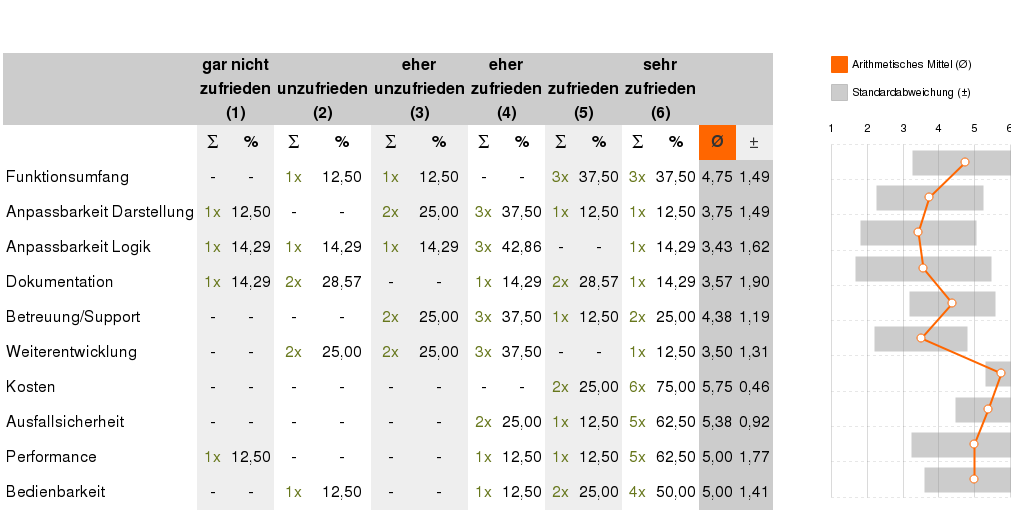
\includegraphics[width=1\linewidth]{images/umfrage_zufriedenheit}
		\caption{Zufriedenheit mit der aktuellen Lösung}
		\label{fig:Umfrage_zufriedenheit}
	\end{figure}

Sehr zufrieden bis zufrieden wurden die Systeme in den Bereichen Kosten ($\varnothing$ 6,0), Ausfallsicherheit ($\varnothing$ 5,83), Performance ($\varnothing$ 5,83), Bedienbarkeit ($\varnothing$ 5,67) und Funktionsumfang ($\varnothing$ 5,50) bewertet. Mit einer Standardabweichung von maximal $\textpm$ 0,55 in diesen Faktoren zeigt sich ein sehr homogenes Bild.
\\
Unterschiede in der Beurteilung werden bei den weiteren Aspekten deutlich. Die Anpassungsmöglichkeiten bezüglich Darstellung ($\varnothing$ 4,33; \textpm 1,03) und Logik ($\varnothing$ 4,20; \textpm 1,10) sowie die Betreuung/Support ($\varnothing$ 4,67; \textpm 1,21) zeigen ein höhere Varianz auch wenn die durchschnittliche Wahrnehmung noch gut ist. Die größten Unterschiede sehen die Hochschulsporteinrichtungen jedoch bei den Themen Dokumentation ($\varnothing$ 3,83; \textpm 1,94) und Weiterentwicklung ($\varnothing$ 3,83; \textpm 1,33). Es ist an dieser Stelle zu bemerken, dass es sowohl zum System BuchSys als auch zum System HSPinONE keine offizielle Dokumentation gibt. Dies mag für HSPinONE im Hinblick auf die Beendigung des Projektes noch nachvollziehbar sein, für ein System wie BuchSys mit hoher Verbreitung ist es jedoch unverständlich. Das die Bewertung hier nicht negativer ausfällt erscheint überraschend, jedoch wurde von den Hochschulsporteinrichtungen angegeben, dass eine grundlegende Dokumentation für das BuchSys System besteht, die aber unter strengen Sicherheitskriterien nur für Kunden zugänglich gemacht wird.
\\
Als eine der kritischen Performance Stellen wurde das Verhalten des Systems zu Anmeldebeginn ausgemacht. Eine Anmeldung im Modus einer \textit{Race Condition} oder \textit{First come, first serve} unterliegt immer der Gefahr bei sehr nachgefragten Inhalten zur Startzeit sehr hohe Nutzerzahlen bedienen können zu müssen. Die Frage nach der Häufigkeit von Beeinträchtigungen zu Anmeldebeginn wurde von 42,9 \% mit gelegentlich, 28,6 \% mit selten und 28,6 \% mit nie beantwortet. Regelmäßige oder immer Beeinträchtigungen wurden nicht genannt. Eine Quantifizierung schwierig und der Grad der Beeinträchtigungsbeurteilung subjektiv geprägt. 71,4 \% der Befragten war jedoch schon von Problemen betroffen (vgl. Abbildung:~\ref{fig:Umfrage_beeinträchtigung}).
	\begin{figure}[h]
		\centering
		\includegraphics[width=0.8\linewidth]{images/umfrage_beeinträchtigung}
		\caption{Häufigkeit der Beeinträchtigung zu Anmeldebeginn}
		\label{fig:Umfrage_beeinträchtigung}
	\end{figure}

Die anschließend Frage ob dafür Anpassungen in der Anmeldung gemacht werden mussten, wurde von 85,7 \% der Einrichtungen mit nein und nur von 14,3 \% mit ja beantwortet. Aus methodischer Sicht ist die Frage in diesem Fall unglücklich gewählt, da in anschließenden Gesprächen eine sehr unterschiedliche Interpretation zur Beantwortung führte. So liegt es im Ermessensspielraum, ob die Auslagerung der Buchungen aus dem verwendeten Content Management System (CMS) zu Anmeldestart eine Anpassung am Anmeldeprozedere ist oder nicht. Ebenso verhält es sich mit der bewussten Staffelung von Anmeldungen über einen gewissen Zeitraum, um die Last zu entzerren.
\\
In der abschließenden Frage der allgemeinen Zufriedenheit antworteten sechs der Befragten mit ihrem System zufrieden zu sein. Nur die Hochschuleinrichtung ohne spezielles System zeigte sich hier unzufrieden mit der aktuellen Lösung.

\subsection{Bewertung der Wichtigkeit von Funktionalitäten}
dafdadfda

\subsection{Zusätzliche Anmerkungen}
adfafdadfadfa


\section{Wichtige Geschäftsprozesse}
\begin{enumerate}
\item Kunden anlegen
\item Kunden verifizieren
\item Kurse anlegen
\item Kurse finden
\item Kurse darstellen
\item Kurse buchen
\item Geld einziehen
\item Rechnungsstellung
\item Teilnehmer informieren
\item Übungsleiter abrechnen
\item Sportstätten vermieten
\item Verträge verwalten
\item Zutritt überprüfen
\item 
\item 
\end{enumerate}
\section{Probleme und Herausforderungen}